% Evaluation de la méthode de la completion/revision des PH
\section{Evaluation}
\label{sec:evaluation}
\subsection{Application: Circadian clock}

In this section we evaluate our approach on learnign the circadian clock actions.
All experiments are run with a ASP implementation of Algorithm \ref{alg:PHC_ap} on a processor Intel Xeon (X5650, 2.67GHz) with 12GB of RAM.

\begin{figure}
\begin{center}
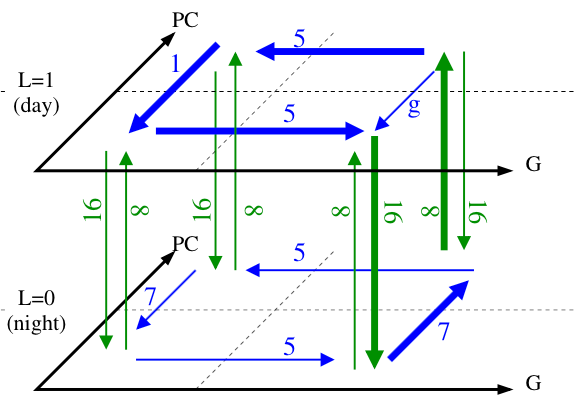
\includegraphics[width=0.4\linewidth]{images/circadianClock-summer.png}
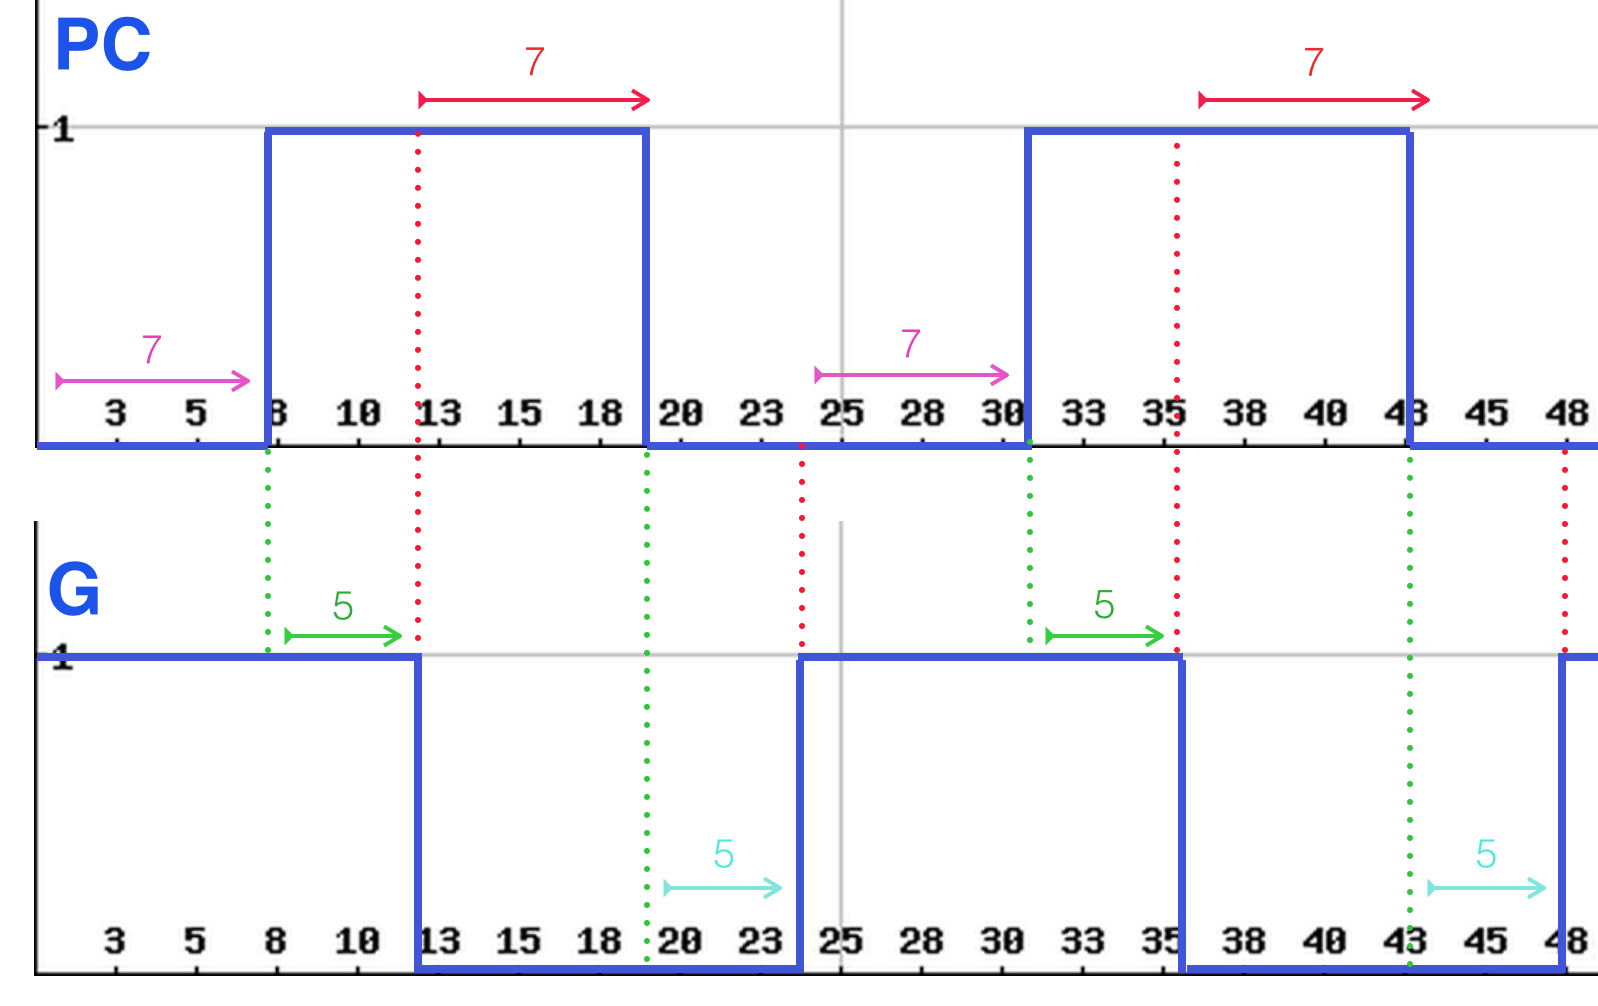
\includegraphics[width=0.4\linewidth]{images/circadianClock-Courb.png}
\end{center}
\caption{The first figure is from \cite{comet2010formal}, it presents the qualitative model of the mammalian circadian cycle during the summer. The second one is a chronogram corresponds to the discretization of the observed data set of a circadian clock components during the night (L=0).}
\end{figure}

\begin{figure}
% TODO: revoir les actions du PH et d'ASP il faut qu'ils soient cohérents

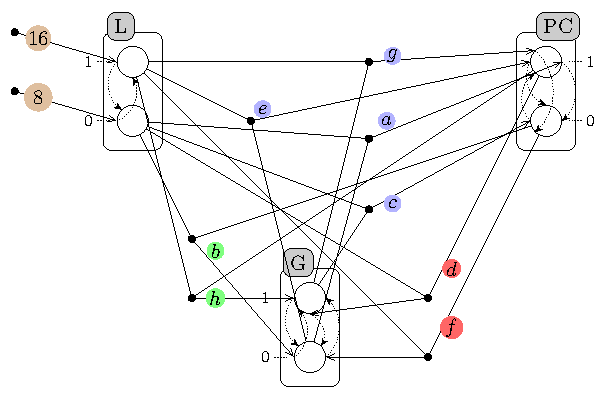
\includegraphics[width=0.4\linewidth]{images/circadianPH.pdf}
%
\hspace{1cm}
%
\begin{minipage}{0.5\linewidth}
	\textbf{Nodes:} \\
\texttt{{\footnotesize process("L",0..1).} }\\
\texttt{{\footnotesize process("PC",0..1).}}\\
\texttt{{\footnotesize process("G",0..1).} }\\

\textbf{Actions:} \\
\texttt{{\footnotesize action("L",0, "L",0,1,  8).}} ~\\
\texttt{{\footnotesize action("L",1, "L",1,0,  16).}} ~\\
\texttt{{\footnotesize action("L",0, "G",0, "PC",1,0,  a).}} ~\\
\texttt{{\footnotesize action("L",0, "PC",0, "G",0,1, b).}} ~\\
\texttt{{\footnotesize action("L",0, "G",1, "PC",0,1, c).}} ~\\
\texttt{{\footnotesize action("L",0, "PC",1, "G",1,0, d).}} \\
\texttt{{\footnotesize action("L",1, "G",0, "PC",1,0,  e).}} ~\\
\texttt{{\footnotesize action("L",1, "PC",0, "G",0,1, f).}} ~\\
\texttt{{\footnotesize action("L",1, "G",1, "PC",1,0, g).}} ~\\
\texttt{{\footnotesize action("L",1, "PC",1, "G",1,0, h).}} 

\end{minipage}
\end{figure}
%
\begin{figure}
\begin{center}
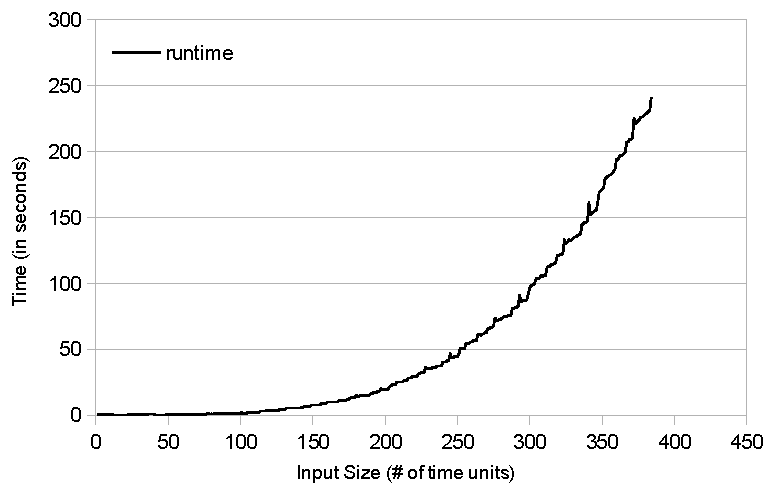
\includegraphics[width=0.6\linewidth]{images/circadian_run_time}
\end{center}
\caption{Run time of the application of Algorithm \ref{alg:PHC_ap} on circadian clock chronograms varying the number of time steps.}
\label{fig:run_time}
\end{figure}

Figure \ref{fig:run_time} show the evolution of run time of our ASP implementation of Algorithm \ref{alg:PHC_ap} on the inference of the circadian clock actions regarding the quantity of input data.
In this experiment we analyse the scalability of our approach by varying the the number of time units of the input, i.e. the size of the chronogram.
Here we can see that the time needed to analyse the input data grows exponentially.
The experiments stop at 384 because the memory required by the ASP solver reached the 12GB of RAM we have.

\subsection{Benchmarks}
